\chapter{Aufbau}
\label{ch:Aufbau}
Dieses Kapitel beschreibt den konkreten Aufbau der Testbench. Wie in Sektion \ref{sec:Architektur und Technologien:Architektur} beschrieben, ist die verwendete Architektur Event-basiert. Abbildung \ref{fig:classDiagram} skizziert eine vereinfachte Form der Testbench in einer UML-Klassendiagramm ähnlichen Form. Aus Übersichtsgründen sind Utility-Klassen, Transfer-Objekte, POJO's\footnote{Plain Old Java Objects: Werden bspw. für die JSON-Deserialisierung benutzt} und die Event-Listener/Event-Publisher der Komponenten nicht Teil des Diagramms. Für jede Komponente, die eine Nachricht in Form eines Events an andere schicken oder von anderen empfangen möchte, existiert ein Listener beziehungsweise ein Publisher. Methoden des Listeners delegieren nach Empfang von Events die erhaltenen Nachrichten (Methodenaufrufe) an ihre nachgeschaltete Komponente. Komponenten die Nachrichten senden wollen, überreichen diese an ihren jeweiligen Publisher, der diese in Form eines Events auf den Event-Bus legt. Näheres ist in Sektion \ref{sec:Aufbau:Events} erklärt. \\
Im Folgenden werden alle wichtigen Systemkomponenten erläutert. Anschließend wird ein Überblick über die verschiedenen Event-Typen gegeben. Danach wir der zeitliche, sich periodisch wiederholende Ablauf eines Intervalls in der Testbench vorgestellt.







%"l, b, r, t"
\begin{figure}[h]
	\centering
	\begin{sideways}
		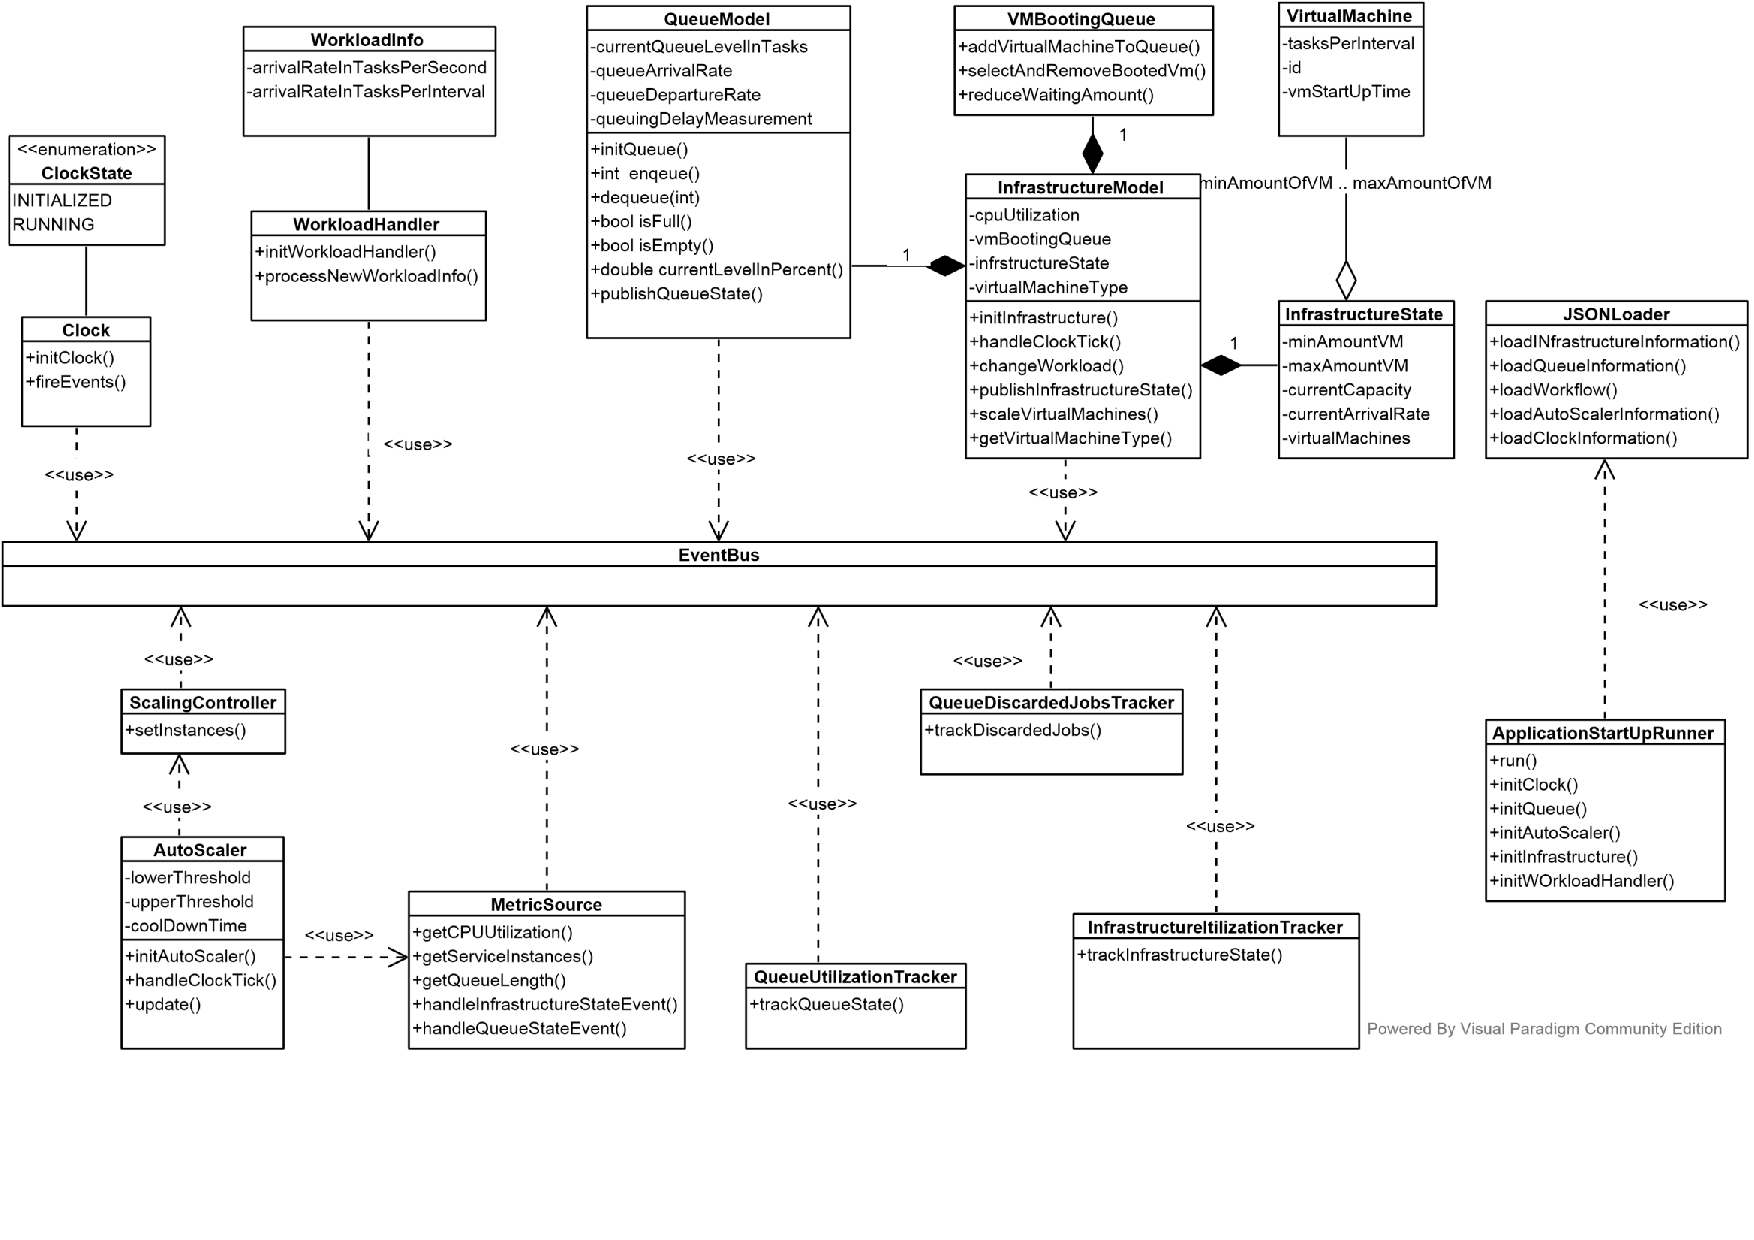
\includegraphics[width=20.0cm, trim={0cm 0cm 0cm 0cm}]{img/classDiagram.pdf}
	\end{sideways}
		\caption{Aufbau des Auto-Skalierers}
	\label{fig:classDiagram}
\end{figure}


\section{Komponenten}
Abbildung \ref{fig:classDiagram} beschreibt den Zusammenhang aller Kern-Komponenten des Auto-Skalierers. Der Event-Bus selbst wird vom Spring-Framework bereitgestellt und ist nicht selbst implementiert. Die \textit{<<use>>} Bezeichnung soll lediglich verdeutlichen, dass die Komponenten Listener und/oder Publisher vorgeschaltet haben, die mit dem Event-Bus interagieren. Aus Gründen der Übersicht existieren keine Assoziations-Pfeile zwischen dem \textit{ApplicationStartUpRunner} und den Komponenten, die er initialisiert. Die Methodennamen lassen aber darauf schließen, mit welcher Komponente noch eine Assoziation existiert.

\subsection{Clock}
\label{sec:aufbau:Clock}
Die \textit{Clock} erfüllt die Aufgabe eines Taktgebers und ist somit das Herz der Testbench. In einer zeit-diskreten Simulation ist es solcher Taktgeber notwendig, da jede Komponenten über den Beginn eines neuen Intervalls informiert werden muss. Dabei gilt: Ein Intervall gilt erst dann als beendet, sobald jede Komponente ihre Aufgaben innerhalb dieses Intervalls erledigt hat. Nach Initialisierung der Komponenten arbeitet die Clock für eine in der Konfiguration definierte Anzahl an Intervallen (Simulationszeit). Dabei wird in jedem Schritt zuerst der Workload, falls notwendig, geändert. Danach versendet die Clock ein Event, dass den Beginn eines neuen Intervalls bekannt gibt. Alle Komponenten werden benachrichtigt und erledigen daraufhin ihre Arbeit, wie Verarbeitung der aktuell anliegenden Workload oder Ausführen von Skalier-Entscheidungen. Abschließend werden \textit{InfrastructureModel} und \textit{QueueModel} durch die Clock aufgefordert ihren aktuellen Zustand zu publizieren. Basierend darauf führen die Komponenten im nächsten Intervall ihre AUfgaben durch. 


\subsection{Infrastructure Model}
Das \textit{InfrastructureModel} bündelt die Haupt-Komponenten der Testbench. Es hat eine Warteschlange für ankommende und wartende Jobs (vgl.\ref{sec:aufbau:QueueModel}), eine Komponente die sich um das Hochfahren der Virtuellen Maschinen kümmert (vgl.\ref{sec:aufbau:BootinQueu}) sowie einen gekapselten Zustand (vgl.\ref{sec:aufbau:State}). \\
Die Information, wie viel Last in welchem Zeitintervall anliegt, wird im \textit{InfrastructureModel} gespeichert und ggf. durch Erhalt einer Workload-Änderung (\textit{changeWorkload()}) geändert. Basierend darauf, ist sie verantwortlich bei Erhalt eines jeden Clock-Ticks (\textit{handleClockTick()}) die erforderliche Menge an Jobs in der Warteschlange (vgl.\ref{sec:aufbau:QueueModel}) einzureihen. Danach berechnet das \textit{InfrastructureModel} als Abstraktion der Infrastruktur die vorhandene Kapazität an Jobs, die in diesem Intervall abgearbeitet werden können (abhängig von Anzahl der vorhandenen Virtuellem Maschinen) und nimmt diese Anzahl aus der Warteschlange und verarbeitet sie. \\
Unregelmäßig muss das Model mit Skalier-Entscheidungen des Auto-Skalieres umgehen (\textit{scaleVirtualMachines()}). Dabei werden hochfahrende Virtuelle Maschinen in der \textit{VMBootingQueue} eingereiht und nach abgelaufener Boot-Zeit mit in die Kapazitäts-Berechnung eingenommen. Das herunterfahren ist einfachheitshalber instantan.\\
Zuletzt kann der Zustand \textit{(vgl.\ref{sec:aufbau:State})} über die Methode \textit{publishInfrastructureState()} publiziert werden. Dieser Vorgang wird wie in Sektion\ref{sec:aufbau:Clock} beschrieben, von \textit{Clock} angestoßen.

\subsubsection{VM Booting Queue}
\label{sec:aufbau:BootinQueu}
Diese Komponente ist eine Warteschlange für hochzufahrende VMs. Nach dem Erhalt einer Skalier-Entscheidung (Hinzufügen einer VM), darf das \textit{InfrastructureModel} diese nicht direkt umsetzen, da eine VM eine gewisse Zeit braucht, um hochzufahren bevor sie aktiv mit in die Kapazitätsberechnung. Deswegen wird eine VM mittels \textit{addVirtualMachineToQueue()} hinzugefügt. In jedem Zeitintervall wird die zu wartende Zeit reduziert und überprüft, ob eine VM bereit ist und zur Menge der aktiv arbeitenden hinzugefügt werden kann \textit{(selectAndRemoveBootedVM())}.  


\subsection{Infrastructure State}
\label{sec:aufbau:State}
Der Zustand der Infrastruktur ist von der Funktionalität abgekapselt. Dieser speichert die aktuell anliegende Workload\textit{(currentArrivalRate)} sowie die aktiven VMs und damit die Kapazität. Der Zustand kann in ein \textit{TransferObject} verpackt und versendet werden. Dieses Objekt beinhaltet zusätzlich Informationen übe die CPU-Auslastung (Diskrepanz zwischen Kapazität und Anzahl der Tasks, die in einem Intervall das System verlassen).

\subsection{Virtual Machine}
\label{sec:aufbau:VM}
Eine Virtuelle Maschine ist eindeutig durch ihre Id identifizierbar. Jede VM benötigt eine vordefinierte Zeit zum hochfahren \textit{vmStartUpTime} und kann pro Zeitintervall eine gewisse Anzahl an Jobs verarbeiten\textit{tasksPerInterval}. Die beiden letzten Werte sind bei dieser Testbench für alle Maschinen pro Simulation gleich, werden also einmalig bei Simulationsstart als Konfigurationsparameter mitgegeben.




\subsection{Auto Scaler}
Der \textit{AutoScaler} als solcher ist kein Teil der Testbench, da er ja das Testobjekt ist. In diesem Fall ist er lediglich hinzugefügt, um die Funktionalität der Testbench zu testen. Ein Auto-Scaler wird angebunden, indem er System-Metriken wie Auslastung oder Warteschlangenlänge über die Komponente \textit{MetricSource} bezieht und Skalierentscheidungen an die Komponente \textit{ScalingController} weiterreicht. Die Interfaces zur Anbindung eines Auto-Skalierers sind in Sektion\ref{sec:Konfiguration:AnbindungScaler} beschrieben.



\subsubsection{Scaling Controller}

\subsubsection{Metric Source}




\subsection{Queue Model}
\label{sec:aufbau:QueueModel}

\subsection{Workload Handler}

\subsubsection{Workload Info}


\subsection{Tracker}

\subsubsection{Queue Utilization Tracker}

\subsubsection{Queue Discarded Jobs Tracker}

\subsubsection{Infrastructure Utilization Tracker}

\subsection{Application Start Up Runner}

\subsection{JSON Loader}

\section{Events}
\label{sec:Aufbau:Events}


\section{Ablauf}



